%
% File acl2020.tex
%
%% Based on the style files for ACL 2020, which were
%% Based on the style files for ACL 2018, NAACL 2018/19, which were
%% Based on the style files for ACL-2015, with some improvements
%%  taken from the NAACL-2016 style
%% Based on the style files for ACL-2014, which were, in turn,
%% based on ACL-2013, ACL-2012, ACL-2011, ACL-2010, ACL-IJCNLP-2009,
%% EACL-2009, IJCNLP-2008...
%% Based on the style files for EACL 2006 by 
%%e.agirre@ehu.es or Sergi.Balari@uab.es
%% and that of ACL 08 by Joakim Nivre and Noah Smith

\documentclass[11pt,a4paper]{article}
\usepackage[hyperref]{acl2020}
\usepackage{booktabs}
\usepackage{graphicx}
\usepackage{times}
\usepackage{latexsym}
\renewcommand{\UrlFont}{\ttfamily\small}

\usepackage{microtype}

\aclfinalcopy % Uncomment this line for the final submission


\newcommand\BibTeX{B\textsc{ib}\TeX}

\title{Deep Learning Approaches for Sentiment Analysis Based on IMDB Movie Reviews}

\author{Lei Yang \\
  Tulane University \\
  {lyang20@tulane.edu} \\\And
  Qinzheng Xu \\
  Tulane University \\
  {qxu5@tulane.edu} \\}

\date{}


\begin{document}
\maketitle
% \begin{abstract}
% Lorem ipsum dolor sit amet, consectetur adipiscing elit, sed do eiusmod tempor incididunt ut labore et dolore magna aliqua. Ut enim ad minim veniam, quis nostrud exercitation ullamco laboris nisi ut aliquip ex ea commodo consequat. Duis aute irure dolor in reprehenderit in voluptate velit esse cillum dolore eu fugiat nulla pariatur. Excepteur sint occaecat cupidatat non proident, sunt in culpa qui officia deserunt mollit anim id est laborum.
% \end{abstract}


\section{Problem Overview}

The issue at hand is using deep learning models to automatically figure out how people feel about movies in reviews. The goal is to correctly find, separate, and label the feelings behind movie reviews from the IMDB database as either positive, negative, or neutral. The subjective and often complicated nature of human language, which includes sarcasm, idiomatic expressions, and different emotional states, makes this job hard. To make things even more difficult, you have to understand the context and semantics of the texts in order to accurately classify the mood. The end goal is to use the information gathered from this research to help entertainment companies improve their services, make their marketing more effective, and make viewers happier. Achieving high accuracy in sentiment analysis can make these insights more open to everyone, so more people can understand and use the feelings and opinions shared in movie reviews.



\section{Data}

This sentiment study is based on information from the IMDB database, which has 50,000 movie reviews. This dataset was carefully chosen for tasks that involve natural language processing and text analytics. Its main focus is on binary mood classification, which means putting reviews into two groups: positive and negative. The data has a lot of it, which makes it a great resource for training and testing deep learning models that are meant to analyse mood. This dataset is unique because it is so big. Compared to other standard datasets in the same field, it lets you train and test models in more ways.

There are two parts to the dataset: a training set and a testing set. Each has 25,000 movie reviews. This fair split makes sure that both positive and negative feelings are represented equally, which is important for teaching computers to correctly sort feelings without any bias. The data comes from the IMDB library and can be found on Kaggle~\citep{maas2011learning}, a website for data science and machine learning projects. In the fields of mood analysis and natural language processing, this makes it easier to repeat studies and make sure that results are correct.


\section{Related Work}

When researchers use sentiment dictionaries to study sentiment analysis, the first thing they need to do is label the expression trend of sentiments. This means that they need to make the emotional meanings of words clearer. The study is based on predefined semantic rules and the sentiment scoring of the lexical expressions in the sentiment dictionary. A series of text processing is used to get the general sentiment tendency of the text. Some researchers, including Tureny et al.~\citep{turney2007anatomy}, look at and figure out how similar words are by adding mutual information intent. They also rebuild the dictionary by adding polar semantics, which makes the dictionary's lexical construction more complex. Yang et al.~\citep{chen2013emotional} start with a sentiment dictionary that already exists and use the LDA model tool to find the topic words in that dictionary. This makes the sentiment tendencies more expressive and gives topic words with multiple meanings a lot of extra information. Pang et al.~\citep{pang2002thumbs} were the first to use machine learning to solve the sentiment analysis binary classification problem. They combined standard bag-of-words methods with machine learning to make the classification work better. Wikarsa et al.~\citep{wikarsa2015text} gathered a huge number of Twitter comments as a dataset and then put emotions into groups based on their meanings. Once the groups were made, the authors used standard machine learning algorithms to figure out how people felt about the tweets, taking into account the emojis and words in the dataset to improve the algorithm's performance and accuracy. Govindarajan et al.~\citep{govindarajan2013sentiment} made a big step forward in combining genetic algorithms and traditional machine learning algorithms in a natural way. They used the combined algorithm as a new way to solve the problem of sentiment binary classification and got better results in binary classification effects. Chikersal et al.~\citep{chikersal2015sentu} changed the emotional rules of emojis and polysemous words in comment texts by mixing rule processing and SVM and processing Twitter corpora. This made text semantic prediction more accurate. But the text opinion research based on machine learning has hit a wall. This is because the research field is getting too big. When it comes to current long text jobs that involve semantics, the combination of dictionary rules and machine learning often doesn't work as planned, which slows down research and development.


\section{Method}

\subsection{Algorithms Used}

We used three different types of neural networks to figure out how people felt about IMDB movie reviews: Artificial Neural Networks (ANN), Recurrent Neural Networks (RNN), and Transformer models. Each of these models takes a different approach to dealing with and making sense of the complex structure of textual data, and each has its own benefits when it comes to catching the subtleties of language and emotion.

\begin{itemize}
    \item \textbf{ANN Model}: As a starting point, the ANN model is used to simulate a sped-up version of the neural processes seen in the human brain. It works by learning patterns and connections in the data through layers of neurones. We used a structure with thick layers and dropout layers in between to keep the model from overfitting and make sure it works well with data it hasn't seen before.
    \item \textbf{RNN Model}: Textual data is usually stored in a certain order, so the RNN model takes that into account when it comes to processing inputs. The RNN can remember long-term relationships thanks to its Long Short-Term Memory (LSTM) units. This makes it perfect for sentiment analysis, where the order and context of words have a big effect on their meaning.
    \item \textbf{Transformer Model}: The Transformer architecture introduces an attention mechanism, allowing the model to focus on different parts of the input sequence when making predictions. This approach is highly effective for understanding context and relationships within the text, offering advantages in processing the complex structure of movie reviews.
\end{itemize}


\subsection{Front-end Interaction Tool}
A Strong open-source Python library Streamlit is praised for its ability to speed up the development of web applications for data science and machine learning. It was designed to provide data scientists and developers more power by enabling them to transform data-centric scripts into minimally coded interactive web apps. Nowadays, there are many different data visualization tools available, each with their own advantages. These include code libraries like Plotly and Bokeh as well as the well-known Tableau and Power BI. However, in the field of interactive applications, Streamlit has become a strong competitor for both developers and data scientists.
The core design principle of Streamlit is simplicity. Just a few lines of Python code can be used to create an interactive web application. A Streamlit program can be created with very little changes from an existing Python script, in contrast to some technologies that need complex settings or dashboard design. Furthermore, Streamlit's instantaneous feedback loop, which allows code modifications to be reflected quickly in the browser, encourages quick prototyping. Compared to programs like Tableau, where iterative design might not be as flexible, this is a benefit.



\subsection{Libraries and Variations}

We used well-known Python tools for deep learning, like TensorFlow and Keras, to put these models into action. These libraries make the development process faster by giving you a lot of tools and features for creating and training neural network models.

\begin{itemize}
    \item We used normal configurations from the Keras library for the ANN and RNN models, but changed the number of units, dropout rates, and sequence processing to make them work best for sentiment analysis.
    \item Because TensorFlow is so flexible, the Transformer model implementation added custom layers and attention mechanisms to make it work for our text classification job.
\end{itemize}

\subsection{Evaluation Methods}

A confusion matrix, which is a powerful way to see how well a model can classify things into different groups, was used to judge the models' success. Accuracy, precision, recall, and the F1 score are some of the key measures we got from the confusion matrix. These metrics give a full picture of how well the model can predict the future and tell the difference between happy and negative emotions.

\begin{itemize}
    \item \textbf{Accuracy} measures the overall effectiveness of the model in correctly identifying sentiments.
    \item \textbf{Precision} and \textbf{Recall} offer insights into the model's ability to correctly predict positive sentiments and minimize false positives.
    \item \textbf{F1 Score} serves as a balance between precision and recall, providing a single metric to assess the model's overall performance in handling both aspects.
\end{itemize}

\subsection{Baselines for Comparison}
A comparison with well-known benchmarks in sentiment analysis was part of our research to make sure that our models worked. By comparing our results to these standards, we wanted to show how our method led to progress and possible improvements. We specifically looked at standard metrics that regular machine learning methods and past neural network models got right in sentiment analysis tasks. We then used these as a starting point to see how much better our ANN, RNN, and Transformer models were.


\section{Preliminary Experiment Results}

\subsection{Label Distribution}

We started our exploratory data analysis by looking at the sentiment label distribution in the dataset. 

\begin{figure}[h]
    \centering
    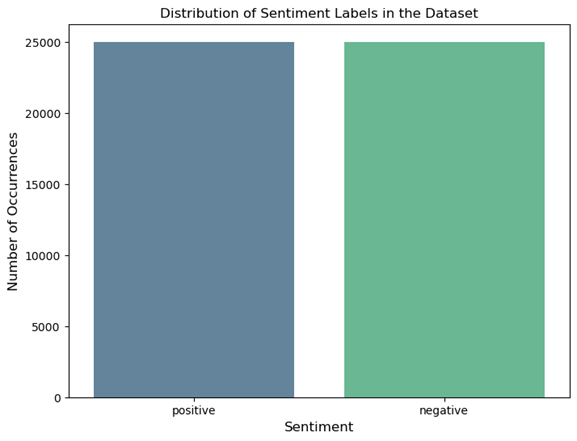
\includegraphics[width=0.4\textwidth]{3.png}
    \caption{Label Distribution}
    \label{fig:polarity_distribution}
\end{figure}


This visualization, which takes the shape of a bar chart, shows how the two sentiment labels—positive and negative—are distributed equally. Each of the two groups has 25,000 occurrences, which is the same amount for both. Because it eliminates the requirement for data balancing strategies and indicates that the dataset is suitable for assessing classification models without running the danger of bias towards a more frequent label, this parity in distribution is helpful for our binary sentiment classification. Given that all classes are equally represented in the dataset, accuracy may also be a trustworthy statistic for assessment.

\subsection{Word Cloud}
A word cloud analysis was part of our exploratory data analysis. It showed us which words were used most often in both the positive and bad movie reviews in our dataset.


\begin{figure}[h]
    \centering
    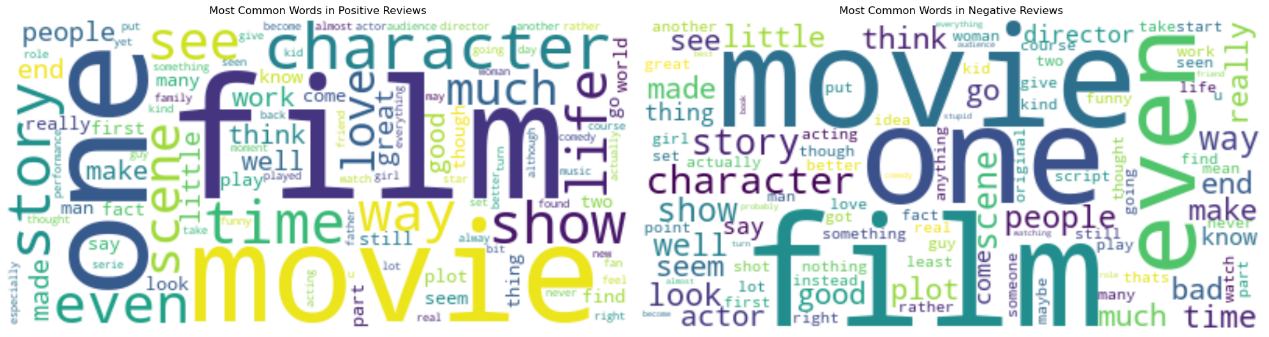
\includegraphics[width=0.4\textwidth]{4.png}
    \caption{Word Cloud for Positive/Negative Reviews}
    \label{fig:polarity_distribution}
\end{figure}

Word clouds show how often a word appears in the evaluations; the bigger a word is, the more often it appears in the evaluations. Positive scores use words like "love," "great," "best," "good," and "amazing" a lot, which shows that people usually say nice things about things. The words "story," "character," and "film" are also used a lot, which shows how important story and character are to good reviews.

The negative rating word cloud, on the other hand, has words like "bad," "worst," "nothing," and "waste," which all make it clear that the user is unhappy. Furthermore, it shows a strong presence of words like "plot," "acting," and "script," which suggest criticism aimed at the movie's acting and story.

The word cloud analysis not only helps you find the most common words, but it also shows you which parts of movies are most often linked to both positive and negative feelings. This information shows the basic ideas and phrases that might be able to tell us how people feel about movies, which could be useful for future work with sentiment analysis and prediction models.





\subsection{Text Features for Extraction}

We will extract the following text features, each offering unique insights into the text data:

\begin{enumerate}
    \item \textbf{Polarity}: This is a measure ranging from -1.0 to 1.0. A score of 0 denotes neutral sentiment, -1 signifies extremely negative sentiment, and +1 reflects highly positive sentiment.
    \item \textbf{Subjectivity}: Expressed as a float within the range of 0.0 to 1.0. A score of 0.0 indicates a highly objective stance, whereas 1.0 suggests a highly subjective viewpoint.
    \item \textbf{Word Count}: The total number of words present in each review.
    \item \textbf{Part-Of-Speech (POS) Tag Ratios}: We will calculate the ratio of specific POS tags to the total word count in a review. The tags include:
    \begin{itemize}
        \item PROPN (Proper Noun), e.g., John, London, NATO.
        \item PUNCT (Punctuation), e.g., ., (, ), ?, !.
        \item NOUN, e.g., woman, tree, beauty.
        \item ADJ (Adjective), e.g., big, yellow, sparkling.
        \item VERB, e.g., eat, running.
    \end{itemize}
    \item \textbf{Uppercase Ratio}: The proportion of uppercase words to the total word count in the review.
    \item \textbf{Digits Ratio}: The proportion of digits to the total word count in the review.
\end{enumerate}

\subsection{Polarity Distribution}
The histogram shows the orientation scores of reviews that are both positive and negative. When reviews are good, the polarity scores are more concentrated on the right side of the scale, reaching their highest point in the range that shows strong positive sentiment. On the other hand, bad reviews have a polarity distribution that leans to the left and has a peak in the negative spectrum. 
\begin{figure}[ht]
    \centering
    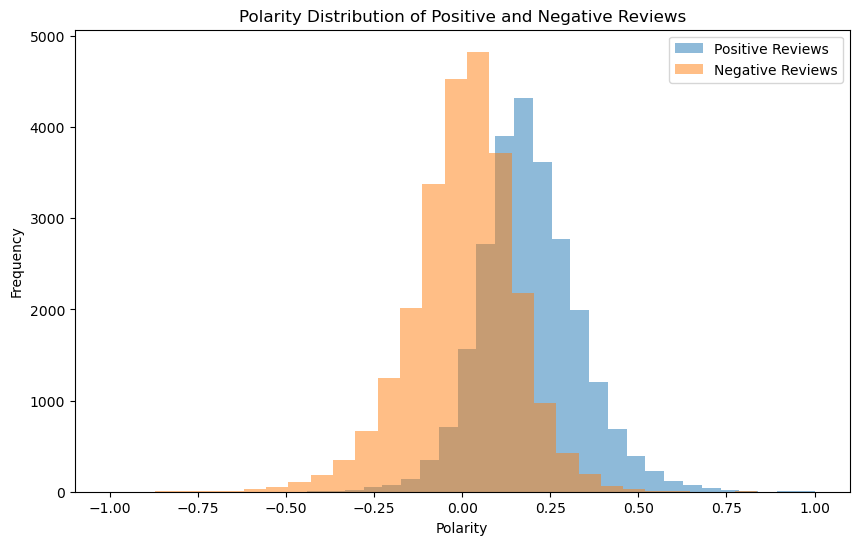
\includegraphics[width=0.5\textwidth]{1.png}
    \caption{Polarity Distribution}
    \label{fig:polarity_distribution}
\end{figure}


The histogram presented captures the polarity scores of both positive and negative reviews. For positive reviews, the polarity scores cluster more densely towards the right side of the scale, peaking in the range that indicates strong positive sentiment. This suggests that the language used in positive reviews is consistently associated with higher positivity in sentiment analysis.

Conversely, the polarity distribution of negative reviews skews towards the left, with a peak in the negative spectrum, underscoring a trend of more negative sentiment expressions. The presence of a few negative reviews with a slightly positive polarity score may indicate either a nuanced view within the reviews or potential noise in the data.
This bimodal distribution highlights the clear demarcation between the sentiments of positive and negative reviews. Understanding the distribution of polarity scores is essential for refining sentiment analysis algorithms, as it demonstrates the typical sentiment range for positive and negative feedback. Such insights can improve the accuracy of sentiment prediction models by emphasizing the polarity features that most strongly correlate with each sentiment category.


\subsection{Word Count Distribution Analysis}
Continuing with our exploratory data analysis, we next turn our attention to the word count distribution within the movie reviews. This analysis is crucial as it provides insights into the verbosity and the level of detail present in the reviews.
\begin{figure}[ht]
    \centering
    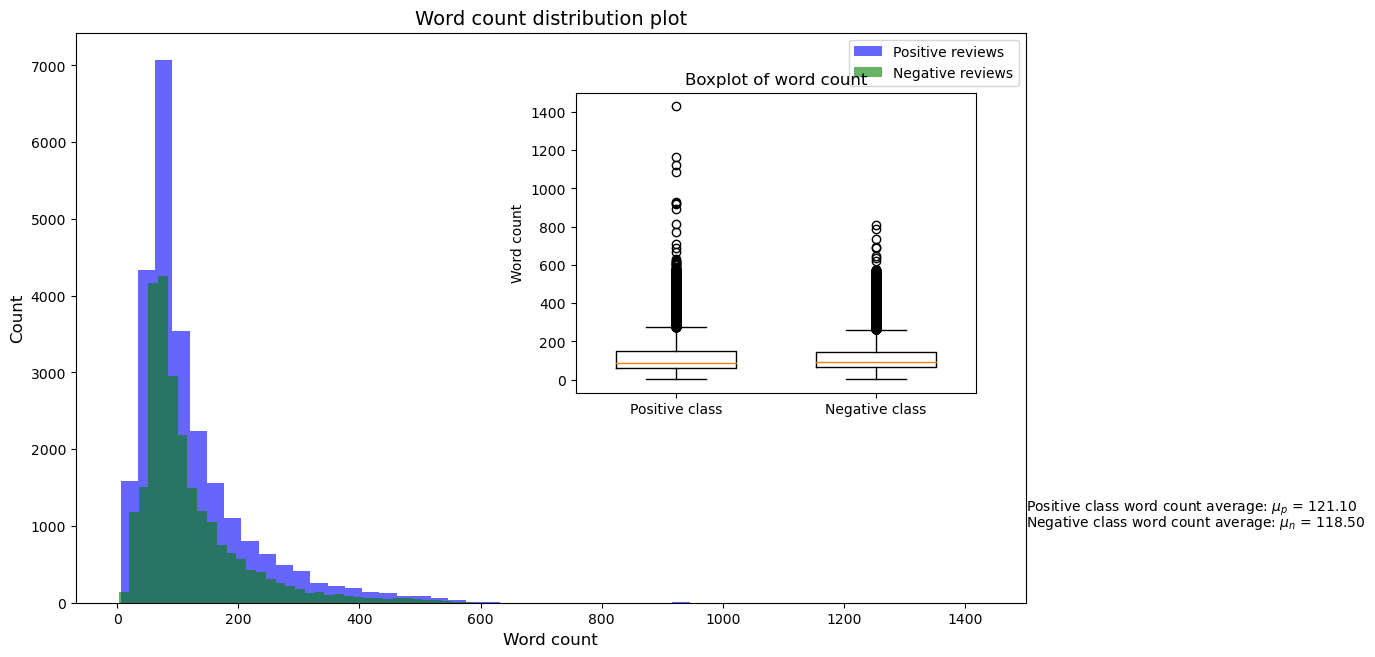
\includegraphics[width=0.5\textwidth]{2.png}
    \caption{Polarity Distribution}
    \label{fig:polarity_distribution}
\end{figure}



\section{Model Training Result}

\subsection{ANN Model}

The performance of the Artificial Neural Network (ANN) model is very good. A confusion matrix shows that there are a lot of true positives and true negatives and almost no false positives and false negatives in the training set. This means that the model is very good at classifying things. The area under the curve (AUC) of the Receiver Operating Characteristic (ROC) curve is 0.99, which means that the models can be separated very well.

The model keeps its good classification accuracy for the testing set, but there are a few more wrong classifications than for the training set. The confusion matrix shows a fair classification, with about the same number of true positives and false negatives. The ROC curve's AUC of 0.94 also shows strong performance. The high AUC is in line with the fact that the accuracy, recall, and F1 scores are almost perfect for the training set. These measures always stay at 0.87 for both classes on the testing set. This is lower than the training set, but it still shows that the model did well on data it had not seen before.


\begin{figure}[ht]
    \centering
    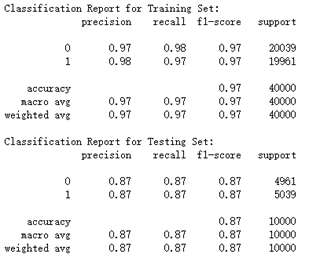
\includegraphics[width=0.5\textwidth]{ann1.png}
    \caption{Evaluation Statistics for ANN Model}
    \label{fig:polarity_distribution}
\end{figure}

\begin{figure}[ht]
    \centering
    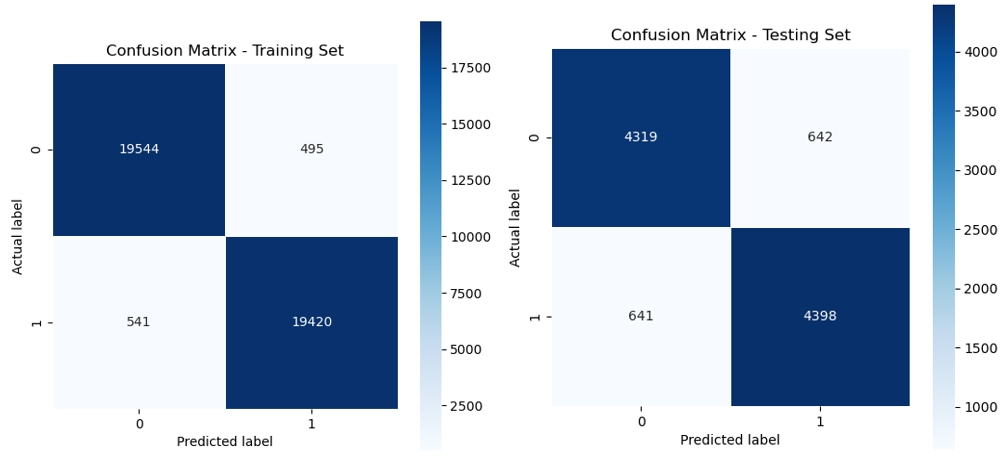
\includegraphics[width=0.5\textwidth]{ann2.png}
    \caption{Confusion Matrices for ANN Model}
    \label{fig:polarity_distribution}
\end{figure}

\begin{figure}[ht]
    \centering
    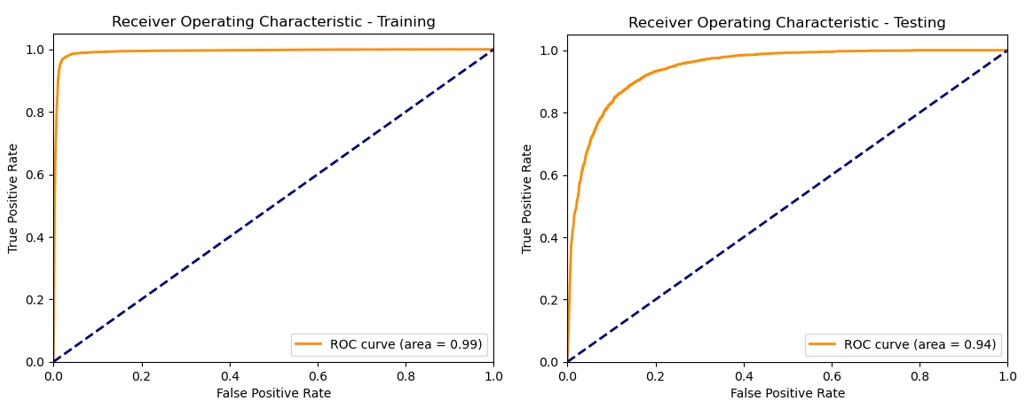
\includegraphics[width=0.5\textwidth]{ann3.png}
    \caption{ROC Curve for ANN Model}
    \label{fig:polarity_distribution}
\end{figure}


\subsection{RNN Model}


\begin{figure}[ht]
    \centering
    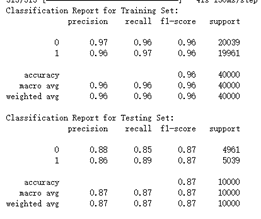
\includegraphics[width=0.5\textwidth]{rnn-1.png}
    \caption{Evaluation Statistics for RNN Model}
    \label{fig:polarity_distribution}
\end{figure}

\begin{figure}[ht]
    \centering
    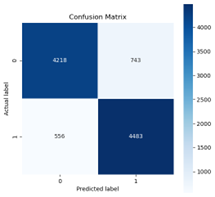
\includegraphics[width=0.5\textwidth]{RNN-2.png}
    \caption{Confusion Matrices for RNN Model}
    \label{fig:polarity_distribution}
\end{figure}

\begin{figure}[ht]
    \centering
    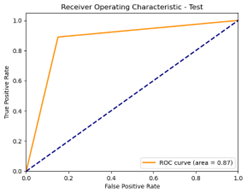
\includegraphics[width=0.5\textwidth]{rnn-3.png}
    \caption{ROC Curve for RNN Model}
    \label{fig:polarity_distribution}
\end{figure}



The performance metrics and visualizations for an LSTM (Long Short-Term Memory) model show that it has been trained to correctly identify two groups (label 0 and label 1) with a high level of accuracy on the training set and a fair level of accuracy on the testing set.
We can see from the confusion matrix that the model got 4218 out of 4483 of the predictions it made on the testing set right. There were, however, 556 false negatives (where it thought label 0 was true label 1) and 743 false positives (where it thought label 1 was true label 0).
With an area under the curve (AUC) of 0.87, the Receiver Operating Characteristic (ROC) graph shows that the model can clearly tell the difference between the two groups. An AUC number close to 1 means that the model works very well, so 0.87 is a pretty good value for many uses.
The classification reports tell us a lot about how well the model worked. The model does a great job on the training set, showing high accuracy, recall, and F1-score for both classes, which stays around 96 percentages. These numbers are a little lower for the testing set, averaging around 87 percentages. This is to be expected, since models tend to do worse on new data that they haven't seen before.


\subsection{Transformer Model}

\begin{figure}[ht]
    \centering
    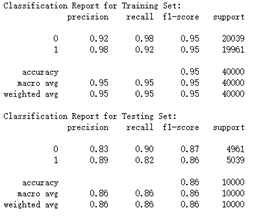
\includegraphics[width=0.5\textwidth]{tran1.png}
    \caption{Evaluation Statistics for Transformer Model}
    \label{fig:polarity_distribution}
\end{figure}

\begin{figure}[ht]
    \centering
    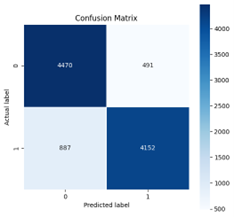
\includegraphics[width=0.5\textwidth]{tran2.png}
    \caption{Confusion Matrices for Transformer Model}
    \label{fig:polarity_distribution}
\end{figure}


The confusion matrix and classification reports show that the Transformer model did well on both the training set and the testing set. Precision and memory did change a bit between the two groups, though. To check if the model was right, the confusion matrix shows that it correctly predicted 4470 instances of class 0 and 4152 instances of class 1. But 491 of the guesses turned out to be wrong. They said that class 0 was class 1 and class 1 was class 0.
To be accurate and remember things, the model got a score of 0.95 for both classes in the training set. Class 1 is a little more accurate than Class 0, but Class 0 is better at remembering things. This proves that the model can reliably change based on the learned facts.
This set of tests shows that class 0 is less accurate than class 1, but class 0 has better memory than class 1. The F1 score for class 0 is 0.87, and the F1 score for class 1 is 0.86. In other words, the model is a little better at finding things that belong to class 0.
With a score of 0.86 on the test set, the Transformer model does pretty well all around. When the tests were given, there was a small difference in the accuracy and recall of the two groups. This suggests that there may be more room for improvement. One way to do this would be to change the decision level or the weights for each class.


\section{Web App Dashboard}

\subsection{Manual Mode}

\begin{figure}[ht]
    \centering
    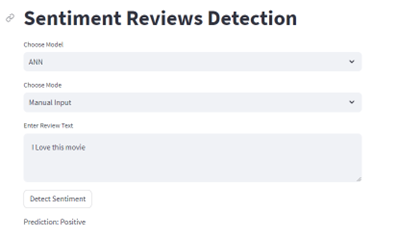
\includegraphics[width=0.5\textwidth]{web1.png}
    \caption{Web Interface with Manual Input}
    \label{fig:polarity_distribution}
\end{figure}

The person using this interface can pick a machine learning model from a dropdown menu. In this case, they picked an Artificial Neural Network (ANN) to study. This time, the method of input was set to "Manual Input" from another drop-down menu.

A text box called "Enter Review Text" is below the dropdowns. This is where the user can write a review of a movie. The example text "I Love this movie" has been written, which means the person likes the movie.

The user can click the "Detect Sentiment" button after writing the review to look at how the review makes them feel. The app uses the chosen ANN model to process the text you enter and shows the outcome below the button. According to the model, the review's sentiment was positive, and the forecast "Positive" backs this up. This matches the positive sentiment in the review text.
This shows that the ANN model correctly figured out how the reviewer felt about the data in this case.

\subsection{CSV Mode}

\begin{figure}[ht]
    \centering
    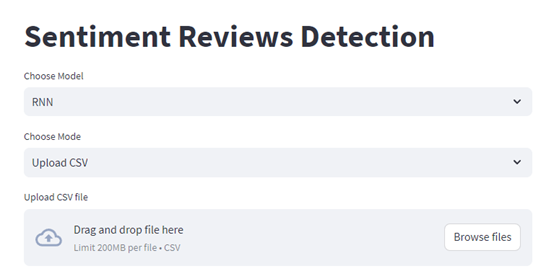
\includegraphics[width=0.5\textwidth]{web2.png}
    \caption{Web Interface with Manual Input}
    \label{fig:polarity_distribution}
\end{figure}

In the CSV file mode. A dropdown menu let the user choose the Recurrent Neural Network (RNN) model. They then posted a CSV file called "test.csv" for sentiment analysis. Once the program has finished processing the file, it shows the sentiment predictions for each review in the file. It shows the outcomes of two reviews in this case, both of which are marked as "Negative." It's likely that these results come from how the RNN model understands the words used in the reviews.

There is a bar chart below the predictions called "Sentiment Count" that shows how many negative reviews were posted. The bar chart shows that there are two reviews, and both have been marked as negative because there is only one bar for the negative count and it is set at a height of 2, which matches the two negative forecasts shown above.

This visual aid makes it easy for users to quickly grasp how the reviews in the CSV file's feelings are spread out. On the other hand, it looks like the X-axis labels on the bar chart are missing or can't be seen. These labels should show the different types of emotion, like "Positive" and "Negative."


\section{Discussion and Conclusion}

\subsection{Discussion}
The results from the Artificial Neural Network (ANN), Recurrent Neural Network (RNN), and Transformer models give a full picture of what mood analysis can do now. Each model did a good job of processing and sorting mood data. The ANN had almost perfect training results, and both the RNN and the Transformer were strong at dealing with complex patterns in sequence data.
The ANN model learned a lot from the training set because it almost always got the right answer and had a high ROC AUC score. But the small drop in speed on the test set makes me wonder if the model might be too good. With its LSTM design, the RNN model also did very well, especially when dealing with sequential text data, which can be hard because of the subtleties of language.
With its attention mechanisms, the Transformer model seems to be very good at capturing contextual connections in data. It kept up its high accuracy and F1-scores, which shows that it could use the training data to make new predictions.


\subsection{Limitations}
Even though the results look good, there are some things that need to be thought about. The difference in accuracy between training and testing shows that the models may be fitting the training data too well. For the Transformer model, the difference in accuracy and recall between the classes also points to possible biases in the model or the data.
It's also possible to get the results wrong because the application's user interface, especially in CSV mode, doesn't have clear labels in the visualizations. Also, the models haven't been tried with a wider range of data or more complex emotions, like sarcasm or irony, which are hard for sentiment analysis models to understand.


\subsection{Conclusion}
Overall, the models that were made are a good base for using mood analysis in other situations. The web app dashboard makes these models easier to use and more accessible by letting you do real-time mood analysis with both manual and CSV inputs.

In future work, fixing the overfitting problem by using regularization techniques or more advanced data addition methods could make the model more stable. It's also important to make the choices made by the models easier to understand, especially for uses that need to know a lot about the model's thinking.The app will be more useful if the user experience is improved so that data can be seen better and more preprocessing is added so that it can handle a wider range of emotions. Transfer learning or multilingual models could also be looked into to make the app more useful in more languages and areas.

As natural language processing and machine learning models keep getting better, it's a great chance to make mood analysis tools even better. In the future, the app can give even more accurate and useful sentiment analysis by using bigger datasets, more complex models, and learning from user feedback.





% \section{Division of Labor and Timeline}

% \subsection{Division of Labor}

% The project tasks have been divided into two main categories: the coding part and the report part. 

% \begin{itemize}
%     \item \textbf{Coding Part:}
%     \begin{itemize}
%         \item \textbf{[name1]} will focus on developing the backend algorithms for sentiment analysis, including the implementation of the neural network models and data preprocessing.
%         \item \textbf{[name2]} is responsible for the frontend development, creating the user interface for the web application and integrating the backend algorithms.
%     \end{itemize}
    
%     \item \textbf{Report Part:}
%     \begin{itemize}
%         \item \textbf{[name1]} will contribute to writing the methodology section of the report, detailing the algorithms used and the rationale behind model choices.
%         \item \textbf{[name2]} will handle the results and discussion sections, analyzing the performance of the implemented models and discussing the implications of the findings.
%     \end{itemize}
% \end{itemize}

% \subsection{Timeline}

% \begin{enumerate}
%     \item \textbf{Frontend Development and Integration:} Completion by [date].
%     \begin{itemize}
%         \item Task involves developing the web application frontend and integrating it with the backend algorithms.
%     \end{itemize}
    
%     \item \textbf{Testing and Refinement:} Completion by [date].
%     \begin{itemize}
%         \item This phase focuses on testing the complete system, refining the models based on performance, and ensuring usability of the web interface.
%     \end{itemize}
    
%     \item \textbf{Final Report Writing:} Completion by [date].
%     \begin{itemize}
%         \item The final step includes compiling the project report, incorporating all sections, and reviewing the document for completeness and accuracy.
%     \end{itemize}
% \end{enumerate}






\bibliography{references}
\bibliographystyle{acl_natbib}


\end{document}
